\Chapter{Review of the literature}{Part I: Microelectronics design}
\label{cha:rol.icdesign}

\begin{summary}
\lipsum[1]
\end{summary}

\section{Introduction}

\section{2D architecture and its limitations}

\section{3D integration}

The benefits of using 3D-ICs are numerous and have been already pointed out in the literature very often over the past few years \cite{659500}. First, by adding vertical dimension to the construction of the physical IC we can increase the IC packaging density. This means more gates for the same circuit footprint, that is much higher functional complexity of the final circuit for the same packaging volume. Secondly, the 3D-SICs are expected to have much better computing/power dissipation ratio. The integration in the 3rd dimension allows the design of circuits with different parts being closer to each other, resulting in less and shorter wires \cite{981091}. Lowering wire delays and allowing higher operating frequencies will result in increased bandwidths between nodes satisfying data hungry applications. Also, less and shorter wires mean lower total parasitic capacitance and inductance of the circuit, resulting in lower power dissipation. Finally, the 3D-SICs will enable the design of really heterogeneous systems, embedding not only traditional digital circuits such as processors and memories, but also analogue circuits such as sensors, antennas and power supplies \cite{4299568}.

Currently different technologies for fabrication of 3D-SICs have been proposed in the literature. Proposed methods have been used for implementation of complete systems going far beyond simple proof-of-concept or feasibility demonstrators. One can mention the implementation of a processor and memory in a single 3D chip dedicated for video coding applications \cite{1696226} and a processor with multiple levels of memory hierarchy dedicated for high-throughput server applications \cite{1168873}. Finally, the first commercial 3D-SIC products have been already announced by IBM \cite{1167715} and companies specialized in 3D semiconductor industry such as Tezzaron \cite{terra04}.

3D Integration is taken into account in the roadmaps of almost all key players in the field of integrated circuit design and manufacturing.

\subsection{3D-SIC advantages}

\subsubsection{Interconnection length}

The 3D integration allows to design circuits with components closer to each other. Wire of a few millimetres long can be replaced by TSV of a few tens of microns \cite{659500}, as shown in Fig. \ref{fig:wire}. These shorter interconnections will introduce shorter delays, hence allowing higher working frequencies.

\begin{figure}[h!]
\begin{center}
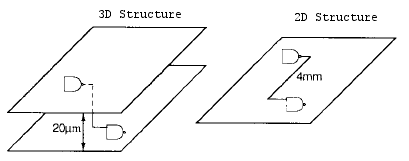
\includegraphics[width=0.75\linewidth]{wire.png}
\end{center}
\vspace{-0.5cm}
\caption{Shorter interconnections}
\label{fig:wire}
\end{figure}

\subsubsection{Silicon efficiency and accessibility}

Adding a vertical dimension allows to increase the integration density. It is therefore possible to have more logic gates than a 2D-IC for the same footprint, hence a more efficient use of the silicon as shown in Fig. \ref{fig:footprint}. For instance, compared to the footprint of a 2D-IC, the 3D-SICs can double the integration for a 50\% use of a 2D footprint \cite{659500}.

\begin{figure}[h!]
\begin{center}
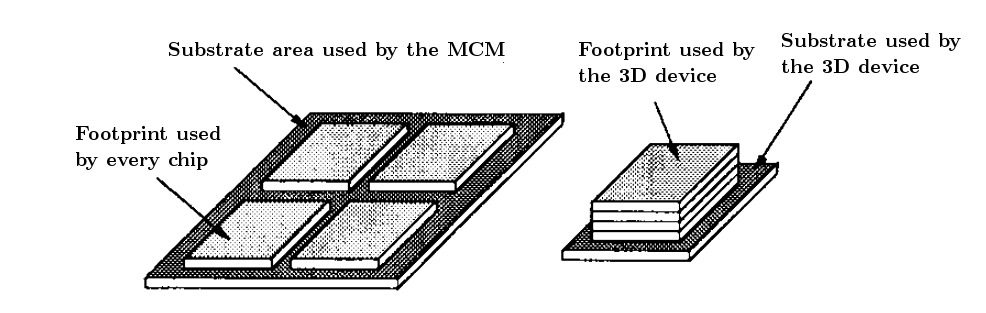
\includegraphics[width=0.75\linewidth]{footprint.png}
\end{center}
\vspace{-0.5cm}
\caption{Silicon efficiency}
\label{fig:footprint}
\end{figure}

In addition, the 3D integration allows a better accessibility for the components, as shown in Fig. \ref{fig:accessibility}. Indeed, for a 2D structure, 8 accessible neighbours can be considered for a central element (Fig. \ref{fig:accessibility} (a)), whereas for a 3D structure, the number of accessible neighbours can reach 116 (Fig. \ref{fig:accessibility} (b)) \cite{659500}.

\begin{figure}[h!]
\begin{center}
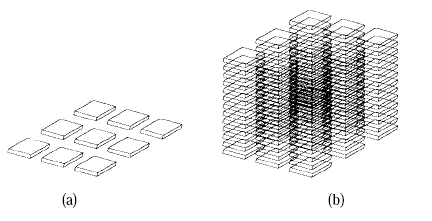
\includegraphics[width=0.75\linewidth]{accessibility.png}
\end{center}
\vspace{-0.5cm}
\caption{Components accessibility}
\label{fig:accessibility}
\end{figure}

\subsubsection{Bandwidth}

The use of TSVs on 3D-SIC can significantly increase the bandwidth of a circuit. Indeed, as shown in Fig. \ref{fig:bandwidth}, the interconnections are not only limited to peripheral connections but can also make use of the circuit's surface. This increase of the bandwidth allows higher working frequencies so that it is easier to satisfy data-heavy applications.

\begin{figure}[h!]
\begin{center}
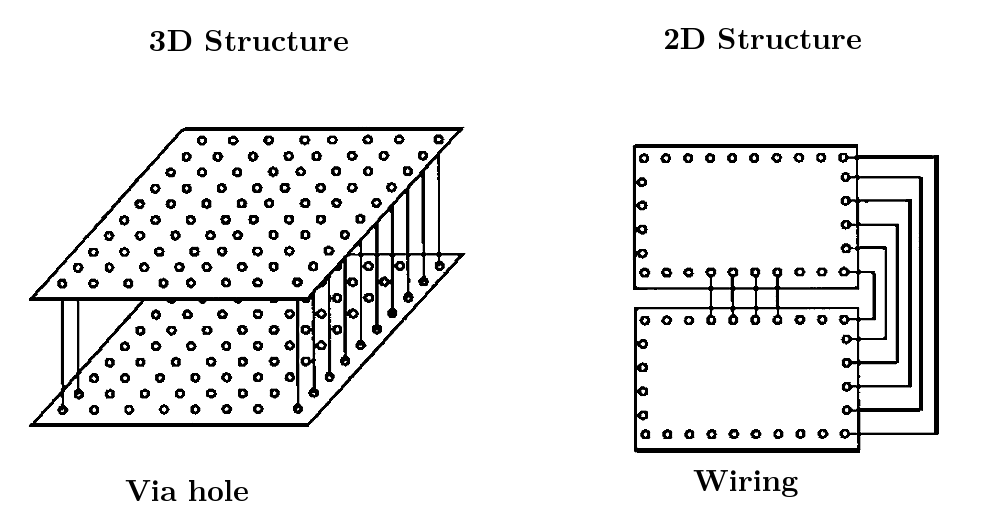
\includegraphics[width=0.75\linewidth]{bandwidth.png}
\end{center}
\vspace{-0.5cm}
\caption{Bandwidth improvement}
\label{fig:bandwidth}
\end{figure}

\subsubsection{Consumption and noise}

Shorter interconnections generally translates into lower capacitance and inductance parasites. This means a decrease of the numbers of repeaters, hence a better consumption, less noise and less jitter.

\subsubsection{Heterogeneous circuits}

The 3D technologies allow truly heterogeneous designs. For instance, it is possible to integrate, in addition to traditional digital circuits of different technologies, analogical circuits such as sensors or antennas, as well as power supply, which give 3D-SIC a high degree diversity \cite{4299568}. The Fig. \ref{fig:heterogeneity} shows a schematic view of a 3D-SIC developed by IMEC for biomedical purposes that contains antennas, DSPs, EEG/ECG sensors, a power supply and solar cells \cite{4198870}.

\begin{figure}[h!]
\begin{center}
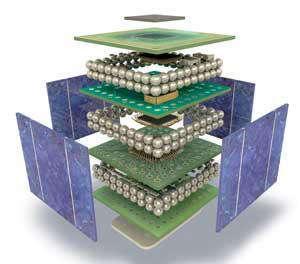
\includegraphics[width=0.5\linewidth]{heterogeneity.png}
\end{center}
\vspace{-0.5cm}
\caption{Schematic illustration of an heterogeneous 3D-SIC (developed by IMEC) \cite{4198870}}
\label{fig:heterogeneity}
\end{figure}

\subsection{Manufacturing technologies}

Several 3D manufacturing technologies have been proposed and have been used to implement complete systems. Among the existing possibilities, four major categories of methods that illustrate 3D integration can be cited \cite{659500,1652906}.

\subsubsection{Chip stacking}

This methods consists in stacking components that have been designed and tested separately to produce a system-in-package (SiP). The vertically-stacked chips are interconnected with traditional wirings. The principal advantage of this method is an improvement in terms of size. The wirings are shorter however the components integration density is not increased compared to a 2D system.

\subsubsection{Transistor stacking}

The transistor stacking consists in creating several transistors level on one substrate. This should be the better way to manufacture 3D circuits although the success rate are currently limited due to thermal issues. The required temperatures to create a layer of high-performance transistors would provoke the destruction of the copper and aluminium already laid down on the previous layer.

\subsubsection{Die-on-wafer stacking}

In this method, known good dies (KGD), which are functional tested chips, are connected to a host wafer containing other KGDs. These KGDs can be interconnected with organic glues, oxide or metal bonding. The wafer and the bonded KGDs are then shaped to create the interconnections. Different substrates can be combined if the required temperature is low enough to minimize non-homogeneous expansion effects.

The die-on-wafer stacking can use interconnections on the edges of the chips or through-die. Depending on the interconnection type, this method can produce a better integration level than the chip stacking, with a better cost per connection ratio and a higher interconnection density, while holding the advantages of the KGDs.

The quality of the stacking depends on the pick-and-place equipment which is used to position the dies on the wafer. The placement accuracy will determine the possible interconnection density. Also, current equipments are supposed to handle fully buffered chips, not naked circuits so it does not provide protection to static discharge. 

\subsubsection{Wafer-level stacking}

This methods consists in bonding entire wafers into a stack. The vertical through-wafer connections are made directly trough each substrate to the next wafer and it transistors layer. Similarly to the previous method, the interconnection density rely on the precision of the alignment, which is however currently better than the die-on-wafer stacking. This greater accuracy implies a better cost per connection ratio and a higher interconnection density compared to the die-on-wafer stacking.

The use of mixed substrates is also possible, only limited by the process temperatures. All the processing is done at the wafer level so wafer handling equipments are used. Since these provide protection to static discharge so there is no need to include buffering between the layers. The methods to bind two wafers are the same that are available for the die-on-wafer method.

One drawback to wafer-level stacking is its efficiency, since the chips on a wafer are not all KGDs.

\subsection{3D-SIC design challenges}

\section{Design flow}

\subsection{2D-IC design flow}

\subsection{3D-SIC design flow}

\section{Design space exploration}

\section{Conclusion}